
%package list
\documentclass{article}
\usepackage[top=3cm, bottom=3cm, outer=3cm, inner=3cm]{geometry}
\usepackage{multicol}
\usepackage{graphicx}
\usepackage{url}
%\usepackage{cite}
\usepackage{hyperref}
\usepackage{array}
%\usepackage{multicol}
\newcolumntype{x}[1]{>{\centering\arraybackslash\hspace{0pt}}p{#1}}
\usepackage{natbib}
\usepackage{pdfpages}
\usepackage{multirow}
\usepackage[normalem]{ulem}
\useunder{\uline}{\ul}{}
\usepackage{svg}
\usepackage{xcolor}
\usepackage{listings}
\lstdefinestyle{ascii-tree}{
    literate={├}{|}1 {─}{--}1 {└}{+}1 
  }
\lstset{basicstyle=\ttfamily,
  showstringspaces=false,
  commentstyle=\color{red},
  keywordstyle=\color{blue}
}
%\usepackage{booktabs}
\usepackage{caption}
\usepackage{subcaption}
\usepackage{float}
\usepackage{array}

\newcolumntype{M}[1]{>{\centering\arraybackslash}m{#1}}
\newcolumntype{N}{@{}m{0pt}@{}}

%%%%%%%%%%%%%%%%%%%%%%%%%%%%%%%%%%%%%%%%%%%%%%%%%%%%%%%%%%%%%%%%%%%%%%%%%%%%
%%%%%%%%%%%%%%%%%%%%%%%%%%%%%%%%%%%%%%%%%%%%%%%%%%%%%%%%%%%%%%%%%%%%%%%%%%%%
\newcommand{\itemEmail}{ }
\newcommand{\itemStudent}{
\newline ALFONSO HUACASI ALEJANDRO SEBASTIAN
\newline CHANCUAÑA ALVIS KLISMANN
\newline CONGONA MANRIQUE MAURICIO ELIAS
\newline FOROCCA MAMANI MAXS SEBASTIAN JOAQUIN}

\newcommand{\itemCourse}{Laboratorio Pweb2}
\newcommand{\itemCourseCode}{}
\newcommand{\itemSemester}{III}
\newcommand{\itemUniversity}{Universidad Nacional de San Agustín de Arequipa}
\newcommand{\itemFaculty}{Facultad de Ingeniería de Producción y Servicios}
\newcommand{\itemDepartment}{Departamento Académico de Ingeniería de Sistemas e Informática}
\newcommand{\itemSchool}{Escuela Profesional de Ingeniería de Sistemas}
\newcommand{\itemAcademic}{2023 - A}
\newcommand{\itemInput}{Del  julio 2023}
\newcommand{\itemOutput}{Al 25 julio 2023}
\newcommand{\itemPracticeNumber}{08}
\newcommand{\itemTheme}{Django Rest Framework}
\newcommand{\itemTeacher}{Ing. Anibal Sardon}

%%%%%%%%%%%%%%%%%%%%%%%%%%%%%%%%%%%%%%%%%%%%%%%%%%%%%%%%%%%%%%%%%%%%%%%%%%%%
%%%%%%%%%%%%%%%%%%%%%%%%%%%%%%%%%%%%%%%%%%%%%%%%%%%%%%%%%%%%%%%%%%%%%%%%%%%%

\usepackage[english,spanish]{babel}
\usepackage[utf8]{inputenc}
\AtBeginDocument{\selectlanguage{spanish}}
\renewcommand{\figurename}{Figura}
\renewcommand{\refname}{Referencias}
\renewcommand{\tablename}{Tabla} %esto no funciona cuando se usa babel
\AtBeginDocument{%
	\renewcommand\tablename{Tabla}
}

\usepackage{fancyhdr}
\pagestyle{fancy}
\fancyhf{}
\setlength{\headheight}{30pt}
\renewcommand{\headrulewidth}{1pt}
\renewcommand{\footrulewidth}{1pt}
\fancyhead[L]{\raisebox{-0.1\height}{
\includegraphics[width=2cm]{src/Imagenes/epis.png}}}
\fancyhead[C]{\fontsize{7}{7}\selectfont	\itemUniversity \\ \itemFaculty \\ \itemDepartment \\ \itemSchool \\ \textbf{\itemCourse}}
\fancyhead[R]{\raisebox{-0.2\height}{
\includegraphics[width=1.2cm]{ima/logo_abet}}}
\fancyfoot[L]{Laboratorio pweb2 }
\fancyfoot[C]{\itemCourse}
\fancyfoot[R]{Página \thepage}

% para el codigo fuente
\usepackage{listings}
\usepackage{color, colortbl}
\definecolor{dkgreen}{rgb}{0,0.6,0}
\definecolor{gray}{rgb}{0.5,0.5,0.5}
\definecolor{mauve}{rgb}{0.58,0,0.82}
\definecolor{codebackground}{rgb}{0.95, 0.95, 0.92}
\definecolor{tablebackground}{rgb}{0.8, 0, 0}

\lstset{frame=tb,
	language=bash,
	aboveskip=3mm,
	belowskip=3mm,
	showstringspaces=false,
	columns=flexible,
	basicstyle={\small\ttfamily},
	numbers=none,
	numberstyle=\tiny\color{gray},
	keywordstyle=\color{blue},
	commentstyle=\color{dkgreen},
	stringstyle=\color{mauve},
	breaklines=true,
	breakatwhitespace=true,
	tabsize=3,
	backgroundcolor= \color{codebackground},
}

\begin{document}  
	
	\vspace*{10px}
	
	\begin{center}	
		\fontsize{17}{17} \textbf{ Informe de Laboratorio \itemPracticeNumber}
	\end{center}
	\centerline{\textbf{\Large Tema: \itemTheme}}
	%\vspace*{0.5cm}	

	\begin{flushright}
		\begin{tabular}{|M{2.5cm}|N|}
			\hline 
			\rowcolor{tablebackground}
			\color{white} \textbf{Nota}  \\
			\hline 
			     \\[30pt]
			\hline 			
		\end{tabular}
	\end{flushright}	

	\begin{table}[H]
		\begin{tabular}{|x{4.7cm}|x{4.8cm}|x{4.8cm}|}
			\hline 
			\rowcolor{tablebackground}
			\color{white} \textbf{Estudiantes} & \color{white}\textbf{Escuela}  & \color{white}\textbf{Asignatura}   \\
			\hline 
   
			{\itemStudent \par \itemEmail} & \itemSchool & {\itemCourse \par Semestre: \itemSemester \par Código: \itemCourseCode}     \\
			\hline 			
		\end{tabular}
	\end{table}		
	
	\begin{table}[H]
		\begin{tabular}{|x{4.7cm}|x{4.8cm}|x{4.8cm}|}
			\hline 
			\rowcolor{tablebackground}
			\color{white}\textbf{Laboratorio} & \color{white}\textbf{Tema}  & \color{white}\textbf{Duración}   \\
			\hline 
			\itemPracticeNumber & \itemTheme & 04 horas   \\
			\hline 
		\end{tabular}
	\end{table}
	
	\begin{table}[H]
		\begin{tabular}{|x{4.7cm}|x{4.8cm}|x{4.8cm}|}
			\hline 
			\rowcolor{tablebackground}
			\color{white}\textbf{Semestre académico} & \color{white}\textbf{Fecha de inicio}  & \color{white}\textbf{Fecha de entrega}   \\
			\hline 
			\itemAcademic & \itemInput &  \itemOutput  \\
			\hline 
		\end{tabular}
	\end{table}
 \begin{table}[H]
		\begin{tabular}{|x{15.3cm}|x{9.8cm}|x{4.8cm}|}
			\hline 
			\rowcolor{tablebackground}
			\color{white}\textbf{Docente}  \\
		  \hline
            \itemTeacher  \\
            \hline
		\end{tabular}
	\end{table}




    \bigskip
    \vspace{80mm}
	\section{Tarea}
	\begin{itemize}		

    \vspace{10mm}
    
        \item En sus grupos de trabajo correspondientes. Elabore un servicio web que tenga un CRUD con el
uso de este framework.
        \item Create - POST.
        \item Read - GET
        \item Update - PUT
        \item Delete - DELETE
        \item Centrarce en el Core business de su aplicaci ́on web. Los m ́as importante y necesario que este
disponible a traves de un servicio web.
        \item Muestre la funcionalidad consumiendola desde el cliente Rest de su preferencia.
        \item El m ́etodo GET puede ser directamente consumido por un navegador web:
        

        \vspace{200mm}
        
      
         
        SOLUCION:
        
        \vspace{10mm}
        \item Explicacion de los archivos de la aplicacion.
        
        \item Archivo admin.py
        
        El código realiza el registro del modelo "Bodega" en la interfaz de administración de Django mediante la función "admin.site.register()". Esto permite acceder y gestionar los objetos del modelo "Bodega" directamente desde el panel de administración del sitio web, facilitando la realización de operaciones CRUD sin necesidad de interactuar directamente con la base de datos.
        \begin{lstlisting}
        from django.contrib import admin
from .models import Bodega
# Register your models here.

admin.site.register(Bodega)

  \end{lstlisting}

    \item Archivo app.py
    
        EEl código configura dos aplicaciones en un proyecto Django, "AplicacionConfig" y "ApiConfig", definiendo el tipo de campo de autoincremento a utilizar y el nombre de cada aplicación.
        \begin{lstlisting}
        from django.apps import AppConfig


class AplicacionConfig(AppConfig):
    default_auto_field = 'django.db.models.BigAutoField'
    name = 'aplicacion'
    
class ApiConfig(AppConfig):
    default_auto_field = 'django.db.models.BigAutoField'
    name = 'api'

  \end{lstlisting}

   \item Archivo models.py
   
        El código define dos modelos de base de datos en Django: "Usuario" y "Bodega". El modelo "Usuario" tiene campos para almacenar información de usuarios, como nombre de usuario, contraseña, correo electrónico, nombres, apellidos y un campo booleano para indicar si es usuario premium. El modelo "Bodega" tiene campos para almacenar información de productos en una bodega, como nombre del cliente, producto, precio y un campo booleano para indicar si está activo.
        \begin{lstlisting}
        from django.db import models

# Create your models here.
class Usuario(models.Model):
    username = models.CharField(max_length= 50)
    password = models.CharField(max_length= 20)
    email = models.EmailField
    nombres = models.CharField(max_length= 200)
    apellidos = models.CharField(max_length= 150)
    isPremium = models.BooleanField(default=False)

class Bodega(models.Model):
    Customer_Name = models.CharField(max_length=100)
    Product = models.CharField(max_length=50)
    Price =  models.PositiveSmallIntegerField()
    is_activate = models.BooleanField(default=True)
  \end{lstlisting}

    
     \item Archivo serializer.py
     
        El código define dos serializadores en Django Rest Framework: "UsuarioSerializer" y "BodegaSerializer". Estos serializadores convierten los modelos "Usuario" y "Bodega" en representaciones JSON y viceversa, permitiendo la serialización y deserialización de los datos para su uso en las API. El "UsuarioSerializer" especifica los campos del modelo "Usuario" que se incluirán en la serialización, mientras que "BodegaSerializer" incluye todos los campos del modelo "Bodega" en la serialización. Además, se ha personalizado el método "create" en "UsuarioSerializer" para crear nuevos objetos de usuario a partir de los datos validados.
        \begin{lstlisting}
        from rest_framework import serializers
from .models import Usuario
from .models import Bodega

class UsuarioSerializer(serializers.ModelSerializer):
    class Meta:
        model = Usuario
        fields = ('username', 'password', 'email','nombres', 'apellidos', 'isPremium')
        
    def create(self, validated_data):
        user = Usuario(**validated_data)
        user.save()
        return user
        
class BodegaSerializer(serializers.ModelSerializer):
    class Meta:
        model = Bodega
        #fields = ('fullname', 'nickname')
        fields = '__all__'
  \end{lstlisting}

     \item Archivo urls.py
     
        El código define las rutas (URLs) para las vistas de una aplicación Django, incluyendo endpoints para el registro, inicio de sesión y página de inicio, y también utiliza el enrutador "DefaultRouter" de Django Rest Framework para generar automáticamente las URLs para las vistas basadas en clases "UsuarioViewSet" y "BodegaViewSet", permitiendo el acceso a las operaciones CRUD para los modelos "Usuario" y "Bodega" a través de la API.
        \begin{lstlisting}
        from django.urls import path, include
from rest_framework import routers
from . import views

router = routers.DefaultRouter()
router.register(r'usuario', views.UsuarioViewSet)
router.register(r'BODEGA', views.BodegaViewSet)


urlpatterns = [
    path('register/', views.register, name='register'),
    path('login/', views.login_view, name='login'),
    path('home/', views.home , name='home'),
    path('', include(router.urls))
    
]
  \end{lstlisting}

     \item Archivo views.py
     
       El código define vistas y viewsets para una aplicación Django con Django Rest Framework. La vista "register" permite el registro de usuarios a través de un formulario y guarda la información en la base de datos. La vista "login view" maneja el inicio de sesión, verificando las credenciales ingresadas por el usuario. La vista "home" muestra la página de inicio después de iniciar sesión exitosamente. Los viewsets "UsuarioViewSet" y "BodegaViewSet" proporcionan operaciones CRUD para los modelos "Usuario" y "Bodega" respectivamente, permitiendo el acceso a través de la API.
        \begin{lstlisting}
        from rest_framework import viewsets, status
from rest_framework.response import Response
from django.shortcuts import render, redirect
from .serializers import UsuarioSerializer
from .models import Usuario
from .serializer import BodegaSerializer
from .models import Bodega


class UsuarioViewSet(viewsets.ModelViewSet):
    queryset = Usuario.objects.all()
    serializer_class = UsuarioSerializer
    
def register(request):
    if request.method == 'POST':
        serializer = UsuarioSerializer(data=request.POST)
        if serializer.is_valid():
            serializer.save()
            return redirect('login')
    else:
        serializer = UsuarioSerializer()

    return render(request, 'register.html', {'serializer': serializer})

def login_view(request):
    if request.method == 'POST':
        passw = request.POST.get('password')
    try:
        user = Usuario.objects.get(username = request.POST.get('username'))
        usname = request.POST.get('username')
        if user.password == passw:
            serializer = UsuarioSerializer(user)
            print("singup")
            request.session['username'] = usname
            return redirect('home')
        else:
            return render(request, 'login.html', {'error_message': 'Credenciales inválidas'})
        print("credencial invalida")
    except Usuario.DoesNotExist:
        return render(request, 'login.html', {'error_message': 'Credenciales inválidas'})
        print("credencial invalida x2")

    return Response({'error': 'Método no permitido'}, status=status.HTTP_405_METHOD_NOT_ALLOWED)

def home(request):
    username = request.session.get('username')
    print("redirigiendo a home")
    return render(request, 'home.html', {'username':username})
    
class BodegaViewSet(viewsets.ModelViewSet):
    queryset = Bodega.objects.all()
    serializer_class = BodegaSerializer
  \end{lstlisting}


   \item Explicacion de los archivos del proyecto
    .
   \item Archivo settings.py
     
       El código configura las aplicaciones y módulos que estarán instalados y activos en un proyecto Django. Incluye aplicaciones esenciales de Django como "admin", "auth", "contenttypes", "sessions" y "messages", junto con otros módulos como "rest framework" para construir APIs, "aplicacion" y "api" para aplicaciones propias del proyecto, y "coreapi" para documentar la API.
        \begin{lstlisting}
        INSTALLED_APPS = [
    'django.contrib.admin',
    'django.contrib.auth',
    'django.contrib.contenttypes',
    'django.contrib.sessions',
    'django.contrib.messages',
    'django.contrib.staticfiles',
    'rest_framework',
    'aplicacion',
    'coreapi', 
    'api'
]

  \end{lstlisting}
  
  El código configura la opción "DEFAULT SCHEMACLASS" en la configuración del framework Django Rest Framework. Establece el esquema de documentación predeterminado como "rest framework.schemas.coreapi.AutoSchema", que utiliza el esquema de documentación automática de CoreAPI para generar la documentación de la API basada en los serializers, viewsets y otros elementos definidos en el proyecto.
  
   \begin{lstlisting}
        REST_FRAMEWORK = {
  'DEFAULT_SCHEMA_CLASS': 'rest_framework.schemas.coreapi.AutoSchema'
}

  \end{lstlisting}

   \item Archivo settings.py
     
       El código configura las URLs del proyecto Django. Define las rutas para acceder a la interfaz de administración de Django a través de "/admin/", las URLs de la aplicación "aplicacion" definidas en "aplicacion.urls", las URLs de la API de la versión 1 definidas en "api.urls", y una ruta para acceder a la documentación de la API generada automáticamente utilizando "rest framework.documentation.include docs urls" a través de "/docs/". Esto permite navegar la interfaz de administración, acceder a las vistas y endpoints de la aplicación y la API, y consultar la documentación de la API en el navegador.
       
        \begin{lstlisting}
        from django.contrib import admin
from django.urls import path, include
from rest_framework.documentation import include_docs_urls

urlpatterns = [
    path('admin/', admin.site.urls),
    path('', include('aplicacion.urls')),
    path('api/v1/', include('api.urls')), 
    path('docs/', include_docs_urls(title='Api Documentation'))
]

  \end{lstlisting}

\item RESULTADOS OBTENIDOS

  
\item[ ]{\raisebox{-0.2\height}{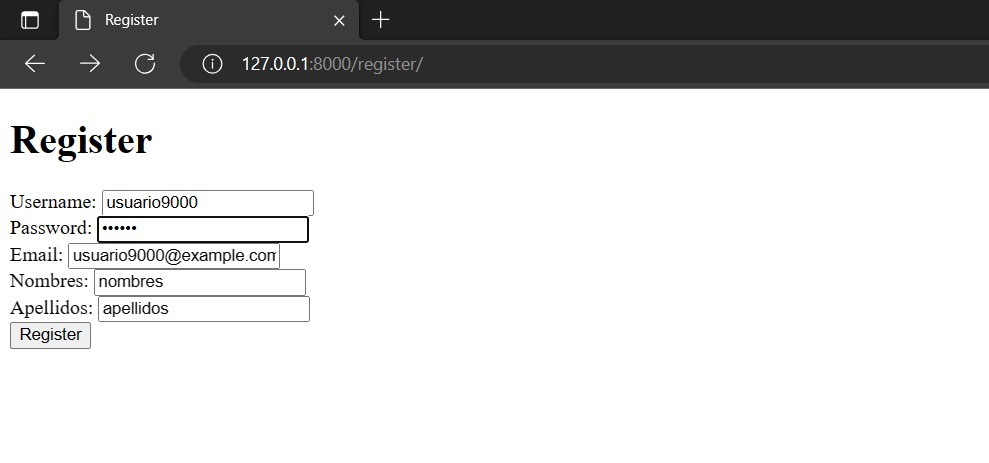
\includegraphics[width=10cm]{src/Imagenes/lab1.png}}}
\item[ ]{\raisebox{-0.2\height}{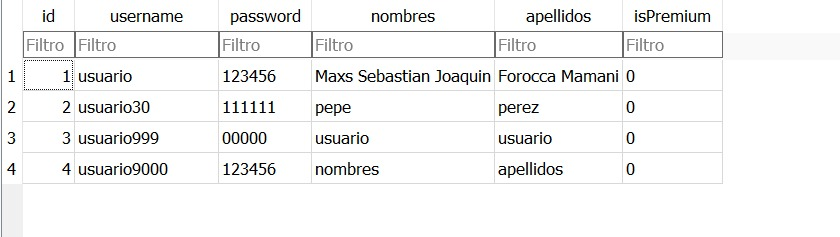
\includegraphics[width=10cm]{src/Imagenes/lab2.png}}}
\item[ ]{\raisebox{-0.2\height}{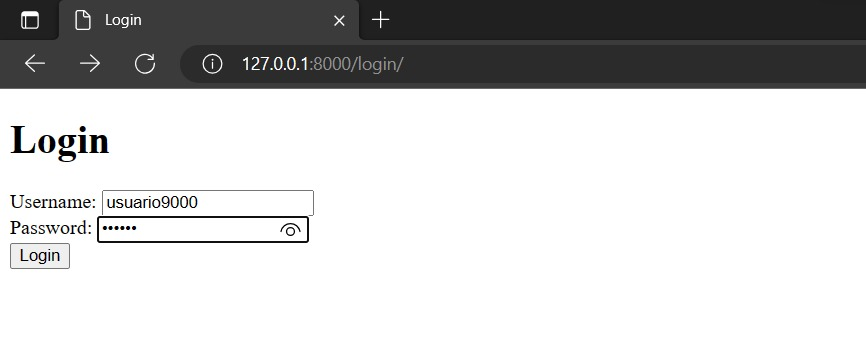
\includegraphics[width=10cm]{src/Imagenes/lab3.png}}}
\item[ ]{\raisebox{-0.2\height}{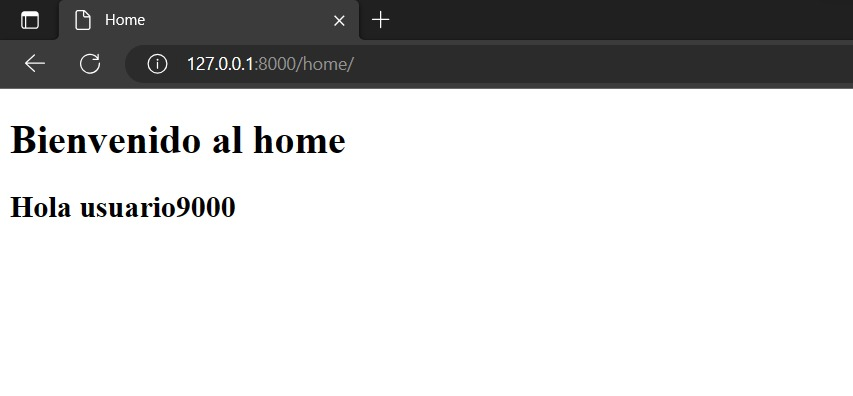
\includegraphics[width=10cm]{src/Imagenes/lab4.png}}}
\item[ ]{\raisebox{-0.2\height}{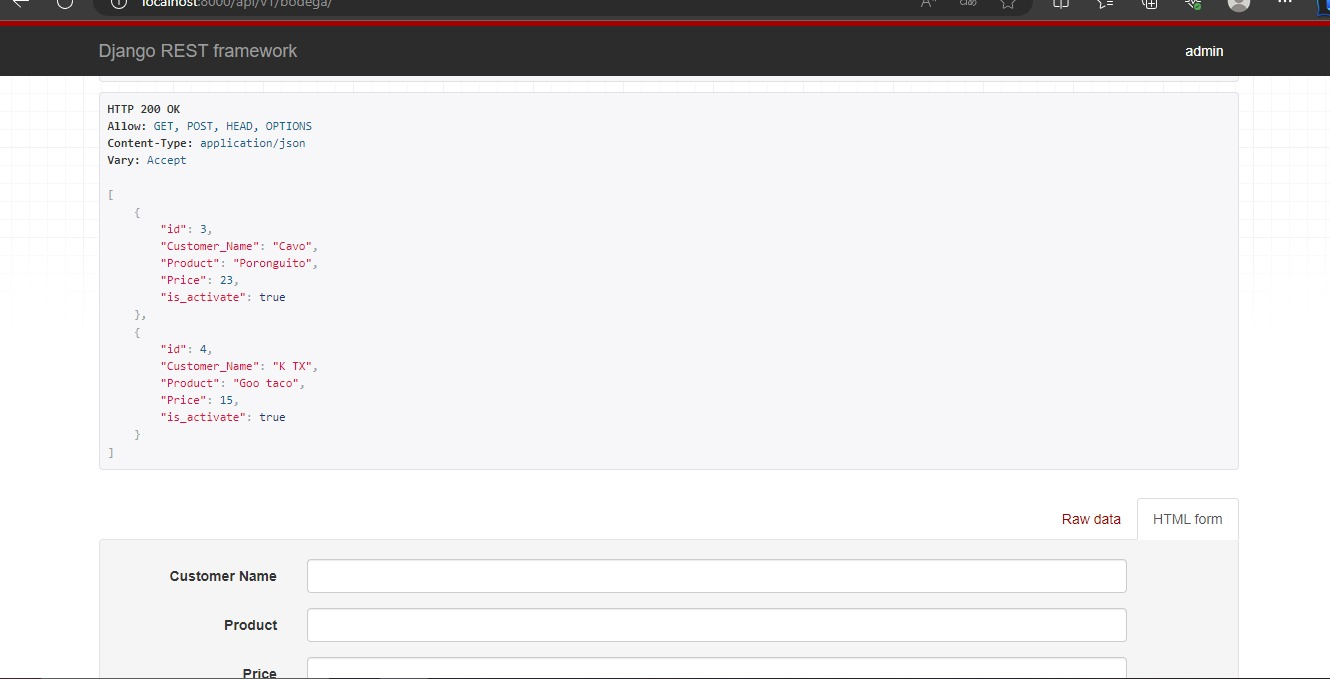
\includegraphics[width=10cm]{src/Imagenes/son1.png}}}
\item[ ]{\raisebox{-0.2\height}{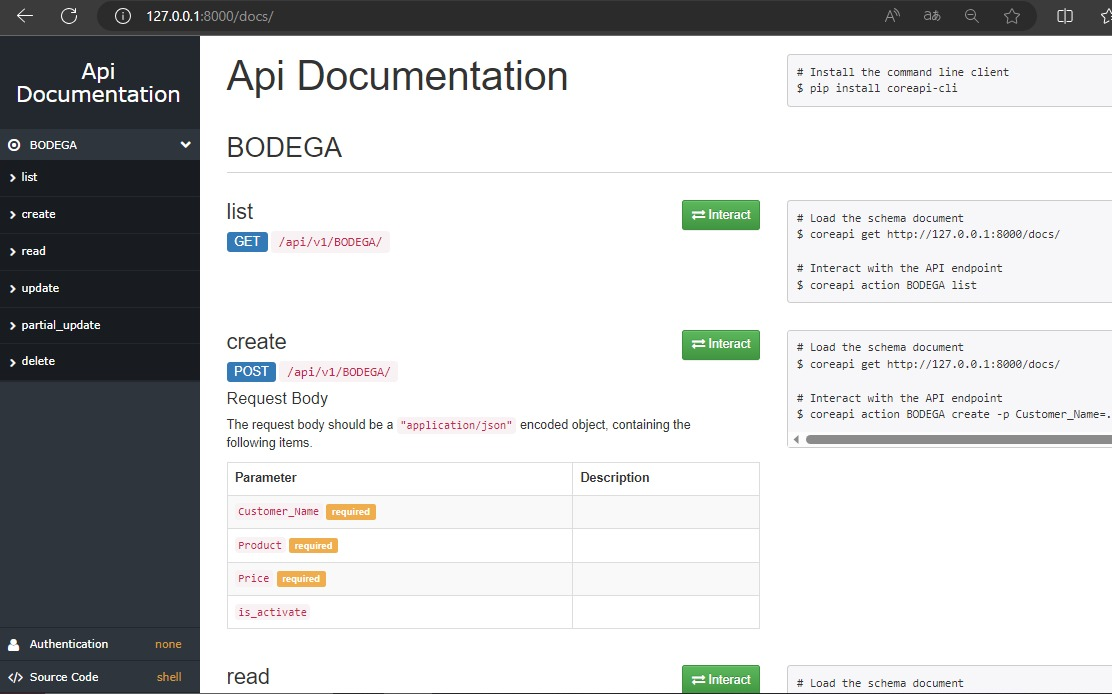
\includegraphics[width=10cm]{src/Imagenes/son2.png}}}
\item[ ]{\raisebox{-0.2\height}{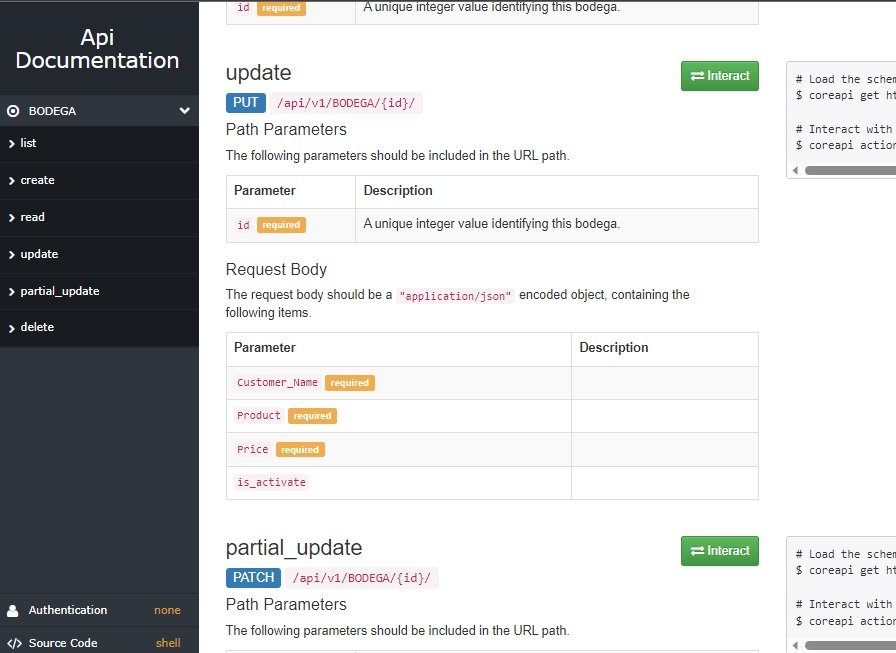
\includegraphics[width=10cm]{src/Imagenes/son3.png}}}

\item COMMITS

\item[ ]{\raisebox{-0.2\height}{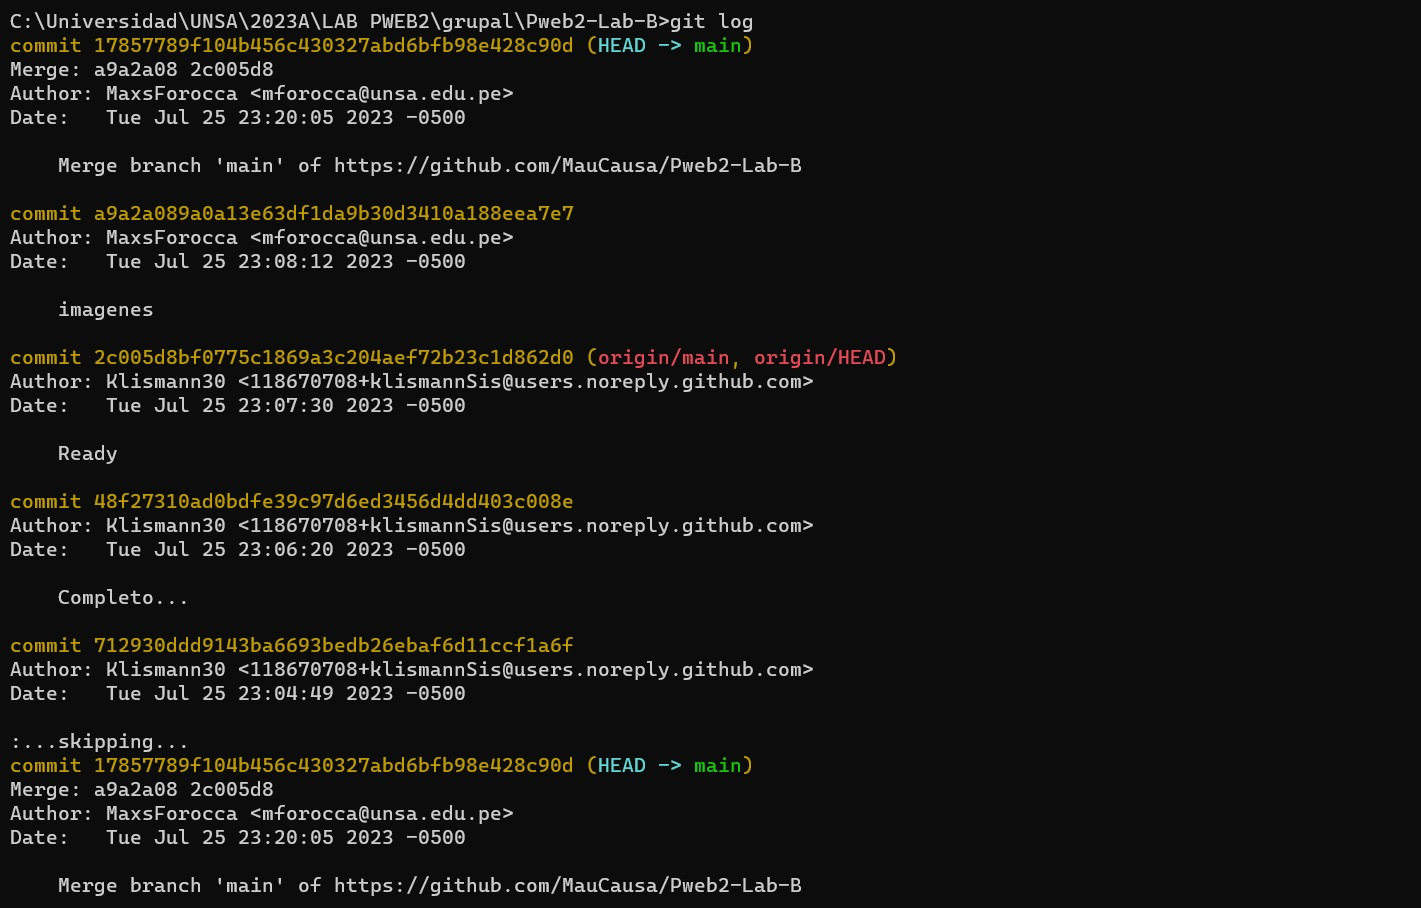
\includegraphics[width=10cm]{src/Commits/comi1.png}}}
\item[ ]{\raisebox{-0.2\height}{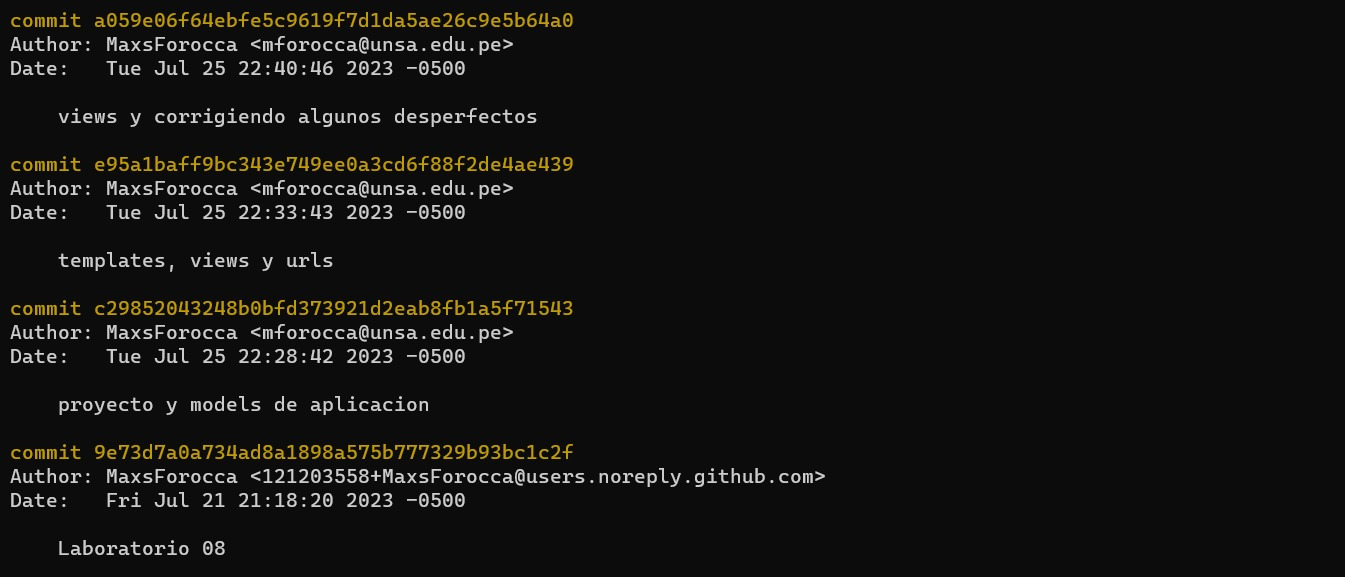
\includegraphics[width=10cm]{src/Commits/comi2.png}}}
\item[ ]{\raisebox{-0.2\height}{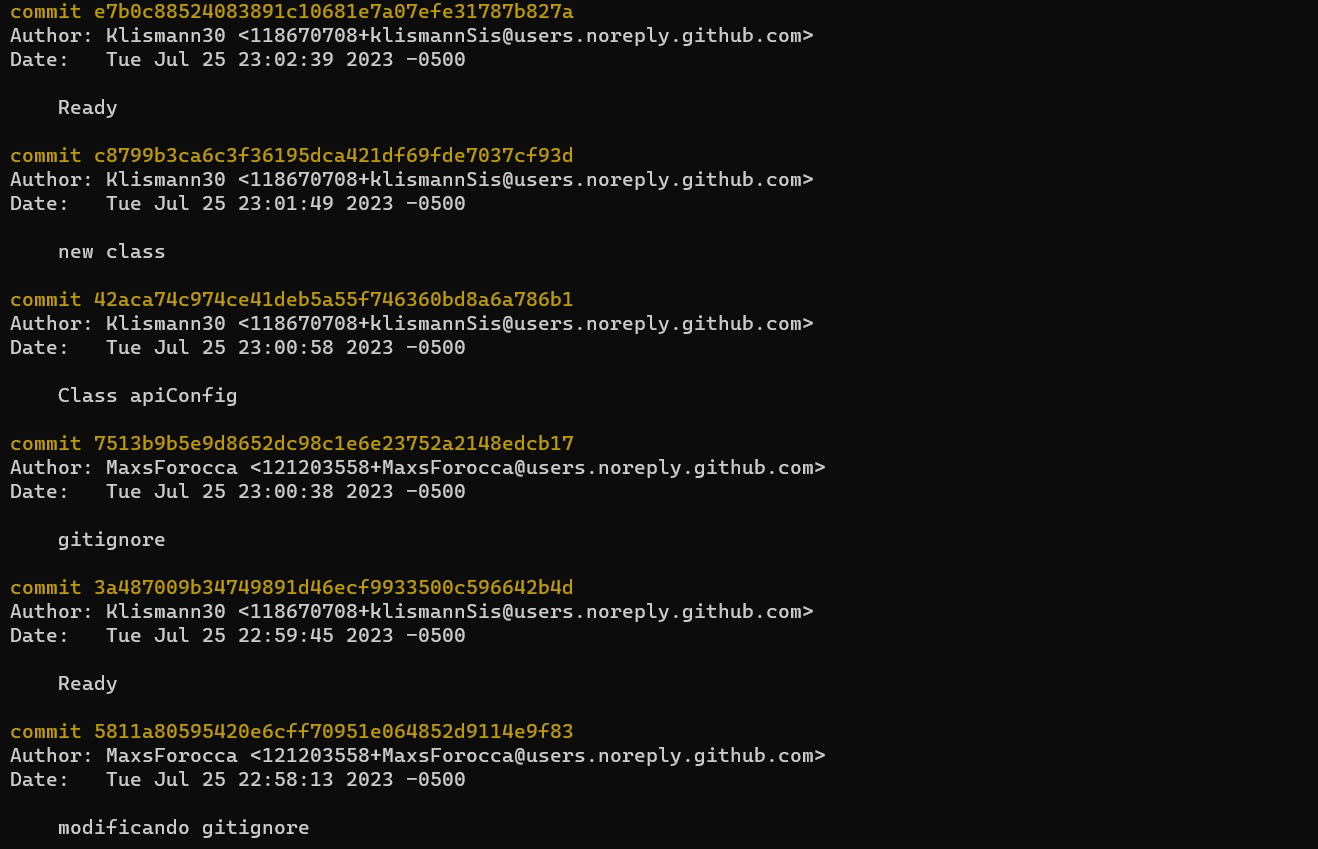
\includegraphics[width=10cm]{src/Commits/comi3.png}}}
\item[ ]{\raisebox{-0.2\height}{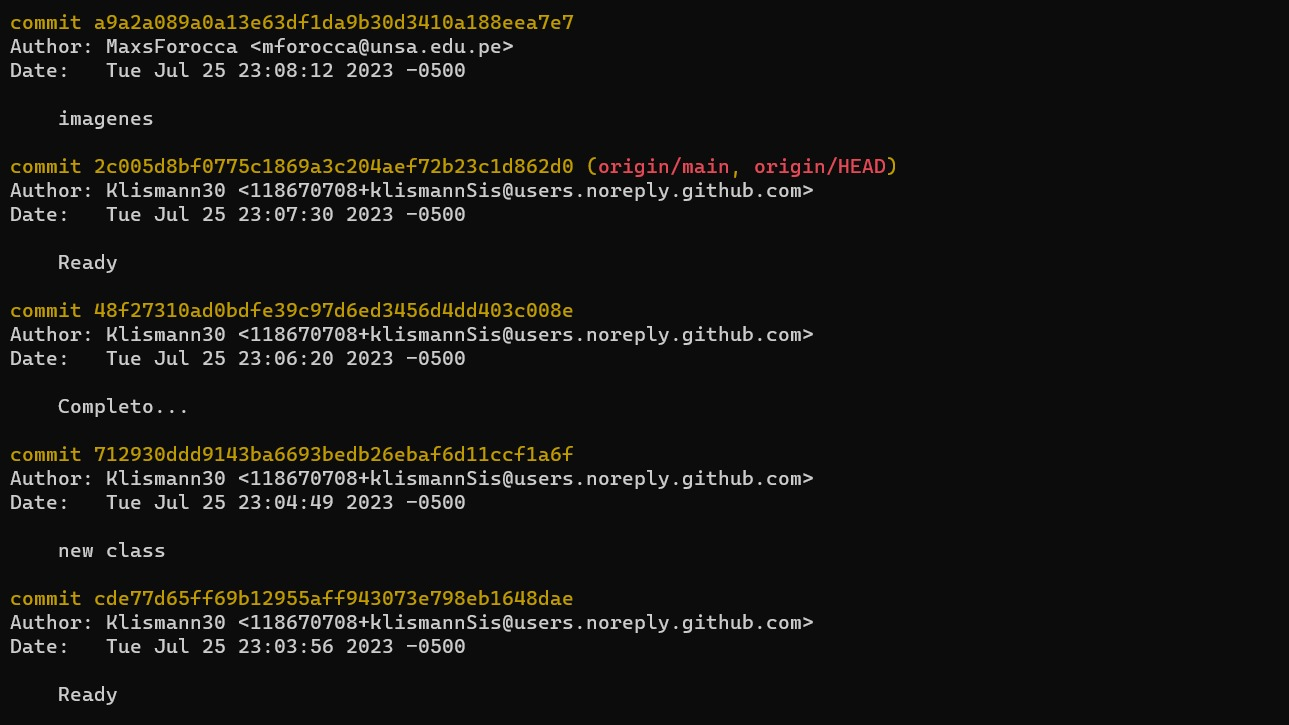
\includegraphics[width=10cm]{src/Commits/comi4.png}}}


   
    
    
    

    \section{} 
     
   
     
    
	\end{itemize} 

  
	\section{URL de Repositorio Github}
	\begin{itemize}
		
	\end{itemize}
		
	\begin{itemize}	
		\item Link del repositorio github
        \item \url{https://github.com/MauCausa/Pweb2-Lab-B/tree/main/Lab08-Informe}
	\end{itemize}


        \vspace{5mm}
   \section{} 
  
    

	
	\subsection{\textcolor{red}{Entregable Informe}}
	\begin{table}[H]
		\caption{Tipo de Informe}
		\setlength{\tabcolsep}{0.5em} % for the horizontal padding
		{\renewcommand{\arraystretch}{1.5}% for the vertical padding
		\begin{tabular}{|p{3cm}|p{12cm}|}
			\hline
			\multicolumn{2}{|c|}{\textbf{\textcolor{red}{Informe}}}  \\
			\hline 
			\textbf{\textcolor{red}{Latex}} & \textcolor{blue}{En conclusion este informe esta editado en latex y en formato PDF.}   \\ 
			\hline 
			
			
		\end{tabular}
	}
	\end{table}

\section{Referencias}
\begin{itemize}			
	\item \url{https://www.django-rest-framework.org/}
	\item \url{https://www.django-rest-framework.org/tutorial/quickstart/}
    \item \url{https://www.django-rest-framework.org/tutorial/1-serialization/}
    \item \url{https://www.django-rest-framework.org/api-guide/authentication/}
\end{itemize}	
	
%\clearpage
%\bibliographystyle{apalike}
%\bibliographystyle{IEEEtranN}
%\bibliography{bibliography}
			
\end{document}